\documentclass{article}\usepackage[]{graphicx}\usepackage[]{color}
%% maxwidth is the original width if it is less than linewidth
%% otherwise use linewidth (to make sure the graphics do not exceed the margin)
\makeatletter
\def\maxwidth{ %
  \ifdim\Gin@nat@width>\linewidth
    \linewidth
  \else
    \Gin@nat@width
  \fi
}
\makeatother

\definecolor{fgcolor}{rgb}{0.345, 0.345, 0.345}
\newcommand{\hlnum}[1]{\textcolor[rgb]{0.686,0.059,0.569}{#1}}%
\newcommand{\hlstr}[1]{\textcolor[rgb]{0.192,0.494,0.8}{#1}}%
\newcommand{\hlcom}[1]{\textcolor[rgb]{0.678,0.584,0.686}{\textit{#1}}}%
\newcommand{\hlopt}[1]{\textcolor[rgb]{0,0,0}{#1}}%
\newcommand{\hlstd}[1]{\textcolor[rgb]{0.345,0.345,0.345}{#1}}%
\newcommand{\hlkwa}[1]{\textcolor[rgb]{0.161,0.373,0.58}{\textbf{#1}}}%
\newcommand{\hlkwb}[1]{\textcolor[rgb]{0.69,0.353,0.396}{#1}}%
\newcommand{\hlkwc}[1]{\textcolor[rgb]{0.333,0.667,0.333}{#1}}%
\newcommand{\hlkwd}[1]{\textcolor[rgb]{0.737,0.353,0.396}{\textbf{#1}}}%

\usepackage{framed}
\makeatletter
\newenvironment{kframe}{%
 \def\at@end@of@kframe{}%
 \ifinner\ifhmode%
  \def\at@end@of@kframe{\end{minipage}}%
  \begin{minipage}{\columnwidth}%
 \fi\fi%
 \def\FrameCommand##1{\hskip\@totalleftmargin \hskip-\fboxsep
 \colorbox{shadecolor}{##1}\hskip-\fboxsep
     % There is no \\@totalrightmargin, so:
     \hskip-\linewidth \hskip-\@totalleftmargin \hskip\columnwidth}%
 \MakeFramed {\advance\hsize-\width
   \@totalleftmargin\z@ \linewidth\hsize
   \@setminipage}}%
 {\par\unskip\endMakeFramed%
 \at@end@of@kframe}
\makeatother

\definecolor{shadecolor}{rgb}{.97, .97, .97}
\definecolor{messagecolor}{rgb}{0, 0, 0}
\definecolor{warningcolor}{rgb}{1, 0, 1}
\definecolor{errorcolor}{rgb}{1, 0, 0}
\newenvironment{knitrout}{}{} % an empty environment to be redefined in TeX

\usepackage{alltt}

\usepackage[margin = 0.5in]{geometry}
\usepackage{float, enumitem}
\usepackage{graphicx}
\usepackage{amsmath}

\setlength{\topsep}{0pt}
\setlength{\parskip}{0pt}
\setlength{\partopsep}{1pt}

\renewcommand\thesubsection{\thesection (\alph{subsection})}
\IfFileExists{upquote.sty}{\usepackage{upquote}}{}
\begin{document}

\title{ASSIGNMENT 7}
\author{Brandon Lampe \\ STAT 527 \\ Advanced Data Analysis I}
\maketitle



\section{ET:}
\subsection{(5 pts) Find a 95\% CI for the proportion p of all adults that favor such a tax hike.}

\begin{knitrout}
\definecolor{shadecolor}{rgb}{0.969, 0.969, 0.969}\color{fgcolor}\begin{kframe}
\begin{alltt}
\hlstd{n} \hlkwb{<-} \hlnum{1014}         \hlcom{# total number of adults surveyed}
\hlstd{p.sup} \hlkwb{<-} \hlnum{0.16}     \hlcom{# proportion of adults surveyed willing to support tax hike}
\hlstd{alpha} \hlkwb{<-} \hlnum{1} \hlopt{-} \hlnum{0.95}
\hlstd{z.crit} \hlkwb{<-} \hlkwd{qnorm}\hlstd{(}\hlnum{1} \hlopt{-} \hlstd{alpha}\hlopt{/}\hlnum{2}\hlstd{)}
\hlstd{SE} \hlkwb{<-} \hlkwd{sqrt}\hlstd{(p.sup}\hlopt{*}\hlstd{(}\hlnum{1} \hlopt{-} \hlstd{p.sup)}\hlopt{/}\hlstd{n)}
\hlstd{L.CI} \hlkwb{<-} \hlstd{p.sup} \hlopt{-} \hlstd{z.crit} \hlopt{*} \hlstd{SE}
\hlstd{U.CI} \hlkwb{<-} \hlstd{p.sup} \hlopt{+} \hlstd{z.crit} \hlopt{*} \hlstd{SE}
\hlstd{L.CI} \hlcom{# lower CI limit}
\end{alltt}
\begin{verbatim}
## [1] 0.1374353
\end{verbatim}
\begin{alltt}
\hlstd{U.CI} \hlcom{# upper CI limit}
\end{alltt}
\begin{verbatim}
## [1] 0.1825647
\end{verbatim}
\end{kframe}
\end{knitrout}

The population paramter ($p$) is the proportion of adults willing to support tax hikes to find extra-terrestrials.  The sample proportion ($\hat{p}$), of the adults surveyed ($n = 1,014$), was 16\%.  With 95\% confidence, the proportion of adults willing to support tax hikes to find extra-terrestrials ($p$) is between 13.7\% and 18.3\%.  This estimate of the CI uses the normal approximation.

\subsection{(5 pts) Suppose it was known that in 1990 that the proportion of all adults willing to support tax hikes to find extra-terrestrials was 0.2. Is there evidence that the proportion of adults in 1997 willing to spring for tax hikes for this purpose has changed since 1990? Carry out a test to answer this
question. Use $\alpha$ = 0.05.}

\begin{knitrout}
\definecolor{shadecolor}{rgb}{0.969, 0.969, 0.969}\color{fgcolor}\begin{kframe}
\begin{alltt}
\hlkwd{prop.test}\hlstd{(p.sup} \hlopt{*} \hlstd{n, n,} \hlkwc{p} \hlstd{=} \hlnum{0.2}\hlstd{,} \hlkwc{correct} \hlstd{=} \hlnum{FALSE}\hlstd{)} \hlcom{# test for equal proportions}
\end{alltt}
\begin{verbatim}
## 
## 	1-sample proportions test without continuity correction
## 
## data:  p.sup * n out of n, null probability 0.2
## X-squared = 10.14, df = 1, p-value = 0.001451
## alternative hypothesis: true p is not equal to 0.2
## 95 percent confidence interval:
##  0.1387246 0.1838418
## sample estimates:
##    p 
## 0.16
\end{verbatim}
\end{kframe}
\end{knitrout}

The null hypothesis is that the proportion of adults willing to support tax hikes to find extral-terresetrials in 1997 ($p$) is equal to 0.2 ($p_0$), which is the proportion of adults supporting this tax in 1990.  That is $H_0: p = p_0$ and the alternative is $H_A : p \ne p_0$.

The test for equal proportions resulted in a p-value of 0.001, which is less than 0.05.  Therefore, I reject the null hypothesis in favor of the alternative.  The proportion of adults willing to support tax hikes to find extra-terrestrials in 1990 is not equal to the proportion of adults willing to support this tax hike in 1997.  Additionally, the confidence interval does for  is: $ 0.138 < p < 0.184$, which does not include $p_0$.

\section{Side effects}

\subsection{(10 pts) Compute an exact upper 95\% confidence bound for the probability of major side e↵ects. Write a short conclusion to your analysis, interpreting the results of the exact bound in the context of the problem.}

\begin{knitrout}
\definecolor{shadecolor}{rgb}{0.969, 0.969, 0.969}\color{fgcolor}\begin{kframe}
\begin{alltt}
\hlcom{# confidence interval from a normal distribution}
\hlstd{n} \hlkwb{<-} \hlnum{15}       \hlcom{# total number of adults surveyed}
\hlstd{p} \hlkwb{<-} \hlnum{0}     \hlcom{# proportion of adults surveyed willing to support tax hike}
\hlstd{alpha} \hlkwb{<-} \hlnum{1} \hlopt{-} \hlnum{0.95}
\hlstd{z.crit} \hlkwb{<-} \hlkwd{qnorm}\hlstd{(}\hlnum{1} \hlopt{-} \hlstd{alpha}\hlopt{/}\hlnum{2}\hlstd{)}
\hlstd{SE} \hlkwb{<-} \hlkwd{sqrt}\hlstd{(p.sup}\hlopt{*}\hlstd{(}\hlnum{1} \hlopt{-} \hlstd{p.sup)}\hlopt{/}\hlstd{n)}
\hlstd{U.CI} \hlkwb{<-} \hlstd{p.sup} \hlopt{+} \hlstd{z.crit} \hlopt{*} \hlstd{SE}
\hlstd{U.CI} \hlcom{# upper CI limit}
\end{alltt}
\begin{verbatim}
## [1] 0.3455249
\end{verbatim}
\begin{alltt}
\hlcom{# Exact binomial test}
\hlkwd{binom.test}\hlstd{(}\hlnum{0}\hlstd{,} \hlnum{15}\hlstd{,} \hlkwc{p} \hlstd{=} \hlnum{0.5}\hlstd{)}
\end{alltt}
\begin{verbatim}
## 
## 	Exact binomial test
## 
## data:  0 and 15
## number of successes = 0, number of trials = 15, p-value =
## 6.104e-05
## alternative hypothesis: true probability of success is not equal to 0.5
## 95 percent confidence interval:
##  0.0000000 0.2180194
## sample estimates:
## probability of success 
##                      0
\end{verbatim}
\end{kframe}
\end{knitrout}

The population parameter ($p$) is the probability of major side effects from using mephetamines to treat children with traumatic brain injuries.  The sample probability ($\hat{p}$) of major side effects was 0\%.  With 95\% confidence, the maximum plausible value for the probability of major side effects from using amphetamines to treat children with traumatic brain injuries is 21.8 \%.

\subsection{(5 pts) What would your reponse be to someone asking you to compute the bound based on the normal distribution, and why?}
Calculation the bound based on the normal distribution is not appropriate.  The bound based on the normal distribution assumes a large sample size and as a rule of thumb is appropriate when (the expected number of successes) $n * p_0 \ge 5$ and (the expected number of failures) $n (1-p_0) \ge 5$.  Additionally, the normal approximation is less reliable for extreme values of $\hat{p}$ (e.g., as the sample proportion approaches zero or unity).

\section{Suicides}

\begin{knitrout}
\definecolor{shadecolor}{rgb}{0.969, 0.969, 0.969}\color{fgcolor}\begin{kframe}
\begin{alltt}
\hlcom{# read data from space delimited text}
\hlstd{suicide} \hlkwb{<-} \hlkwd{read.table}\hlstd{(}\hlkwc{text}\hlstd{=}\hlstr{"
  Month  Suicides
  01Jan      1867
  02Feb      1789
  03Mar      1944
  04Apr      2094
  05May      2097
  06Jun      1981
  07Jul      1887
  08Aug      2024
  09Sep      1928
  10Oct      2032
  11Nov      1978
  12Dec      1859
"}\hlstd{,} \hlkwc{header}\hlstd{=}\hlnum{TRUE}\hlstd{,} \hlkwc{stringsAsFactors} \hlstd{=} \hlnum{FALSE}\hlstd{)}

\hlstd{suicide}\hlopt{$}\hlstd{prop} \hlkwb{<-} \hlstd{suicide}\hlopt{$}\hlstd{Suicides} \hlopt{/} \hlkwd{sum}\hlstd{(suicide}\hlopt{$}\hlstd{Suicides)} \hlcom{# calculate proportions}
\hlstd{suicide}\hlopt{$}\hlstd{prop.eq} \hlkwb{<-} \hlstd{(}\hlkwd{sum}\hlstd{(suicide}\hlopt{$}\hlstd{Suicides)}\hlopt{/}\hlnum{12}\hlstd{)} \hlopt{/} \hlkwd{sum}\hlstd{(suicide}\hlopt{$}\hlstd{Suicides)} \hlcom{# calculate equal proportions}
\hlkwd{sum}\hlstd{(suicide}\hlopt{$}\hlstd{prop)} \hlcom{# check that sum is equal to 1}
\end{alltt}
\begin{verbatim}
## [1] 1
\end{verbatim}
\end{kframe}
\end{knitrout}

\begin{knitrout}
\definecolor{shadecolor}{rgb}{0.969, 0.969, 0.969}\color{fgcolor}\begin{kframe}
\begin{alltt}
\hlcom{# calculate chi-square goodness-of-fit}
\hlstd{x.summ} \hlkwb{<-} \hlkwd{chisq.test}\hlstd{(suicide}\hlopt{$}\hlstd{Suicides,} \hlkwc{correct} \hlstd{=} \hlnum{FALSE}\hlstd{,} \hlkwc{p} \hlstd{= suicide}\hlopt{$}\hlstd{prop.eq)}
\hlstd{x.summ}
\end{alltt}
\begin{verbatim}
## 
## 	Chi-squared test for given probabilities
## 
## data:  suicide$Suicides
## X-squared = 51.7905, df = 11, p-value = 2.975e-07
\end{verbatim}
\begin{alltt}
\hlstd{x.table} \hlkwb{<-} \hlkwd{data.frame}\hlstd{(}\hlkwc{month} \hlstd{= suicide}\hlopt{$}\hlstd{Month,}
                      \hlkwc{obs} \hlstd{= suicide}\hlopt{$}\hlstd{Suicides,}
                      \hlkwc{exp} \hlstd{= x.summ}\hlopt{$}\hlstd{expected,}
                      \hlkwc{res} \hlstd{= x.summ}\hlopt{$}\hlstd{residuals,}
                      \hlkwc{chisq} \hlstd{= x.summ}\hlopt{$}\hlstd{residuals}\hlopt{^}\hlnum{2}\hlstd{,}
                      \hlkwc{stdres} \hlstd{= x.summ}\hlopt{$}\hlstd{stdres)}

\hlstd{x.table.long} \hlkwb{<-} \hlkwd{melt}\hlstd{(x.table,} \hlkwc{id.vars} \hlstd{=} \hlkwd{c}\hlstd{(}\hlstr{"month"}\hlstd{),} \hlkwc{measure.vars} \hlstd{=} \hlkwd{c}\hlstd{(}\hlstr{"obs"}\hlstd{,} \hlstr{"exp"}\hlstd{),}
                     \hlkwc{variable.name} \hlstd{=} \hlstr{"stat"}\hlstd{,} \hlkwc{value.name} \hlstd{=} \hlstr{"value"}\hlstd{)}
\end{alltt}
\end{kframe}
\end{knitrout}

This analysis was formulated as a goodnes-of-fit test.  The plausibility of a constant suicide rate per month was tested by comparing the proportions of the estimated (observed) suicides each month to the hypothesized proportion (sum of suicides divided by 12 months).  The null hypothesis was that each month had a proportion of suicides equal to the hypothesized proportion; that is $H_0: p_1 = p_{01}, p_2 = p_{02}, ..., p_{12} = p_{012}$; and $H_A:$ not $H_0$.

The p-value from the Chi-squared test was $2.98e^{-7}$; therefore, at the 5\% level I reject the null hypothesis in favor of the alternative.  That is, it is not plausible that the suicide rate is constant.  Comparisons between the expected and observed suicide counts are shown below along with the respective Chi-squared values for each month.  From these data, it is apparent that February, May, and April have high Chi-squared values that do not agree with the null hypothesis.

\begin{knitrout}
\definecolor{shadecolor}{rgb}{0.969, 0.969, 0.969}\color{fgcolor}\begin{kframe}
\begin{alltt}
\hlcom{#create bar plot comparing recorded to expected suicides by month}
\hlstd{s.bar} \hlkwb{<-} \hlkwd{ggplot}\hlstd{(x.table.long,} \hlkwd{aes}\hlstd{(}\hlkwc{x} \hlstd{= month,} \hlkwc{fill} \hlstd{= stat,} \hlkwc{weight} \hlstd{= value))}
\hlstd{s.bar} \hlkwb{<-} \hlstd{s.bar} \hlopt{+} \hlkwd{geom_bar}\hlstd{(}\hlkwc{position} \hlstd{=} \hlstr{"dodge"}\hlstd{)}
\hlstd{s.bar} \hlkwb{<-} \hlstd{s.bar} \hlopt{+} \hlkwd{labs}\hlstd{(}\hlkwc{xlab} \hlstd{=} \hlstr{"Month"}\hlstd{,} \hlkwc{title} \hlstd{=} \hlstr{"observed and expected suicide rates"}\hlstd{)}
\hlstd{s.bar}
\end{alltt}
\end{kframe}

{\centering 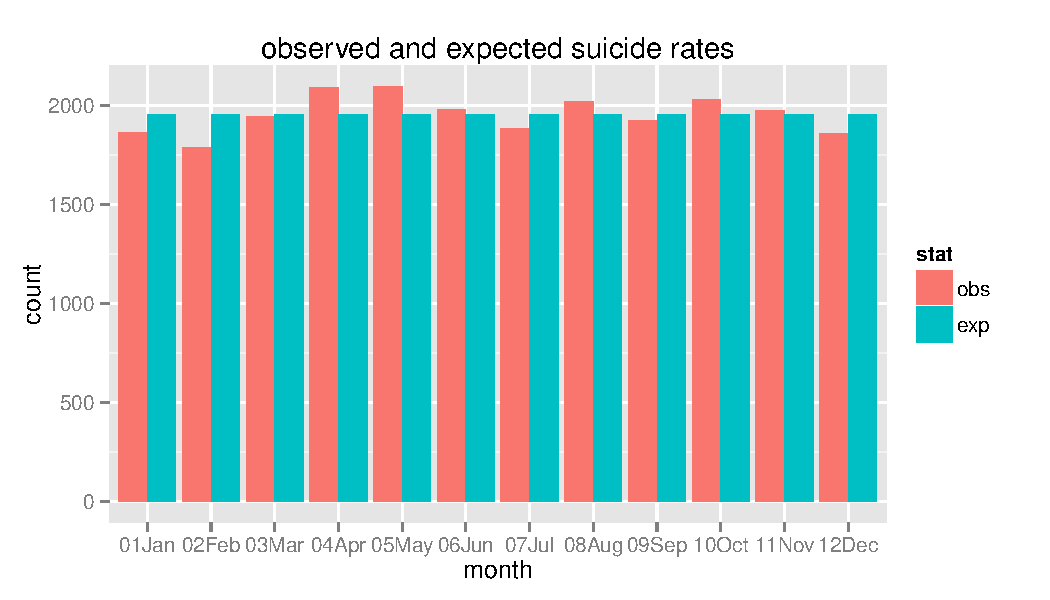
\includegraphics[width=\maxwidth]{figure/3_plot-1} 

}


\begin{kframe}\begin{alltt}
\hlstd{x.table.chisq} \hlkwb{<-} \hlstd{x.table[,}\hlkwd{c}\hlstd{(}\hlstr{"month"}\hlstd{,} \hlstr{"chisq"}\hlstd{)]}
\hlstd{x.table.chisq}\hlopt{$}\hlstd{month} \hlkwb{<-} \hlkwd{with}\hlstd{(x.table,} \hlkwd{reorder}\hlstd{(month,} \hlopt{-}\hlstd{chisq))}

\hlcom{# create bar plot showing contribution of chi-sq}
\hlstd{p} \hlkwb{<-} \hlkwd{ggplot}\hlstd{(x.table.chisq,} \hlkwd{aes}\hlstd{(}\hlkwc{x} \hlstd{= month,} \hlkwc{weight} \hlstd{= chisq))}
\hlstd{p} \hlkwb{<-} \hlstd{p} \hlopt{+} \hlkwd{geom_bar}\hlstd{()}
\hlstd{p} \hlkwb{<-} \hlstd{p} \hlopt{+} \hlkwd{labs}\hlstd{(}\hlkwc{title} \hlstd{=} \hlstr{"Contribution to Chi-sq statistic"}\hlstd{)}
\hlstd{p} \hlkwb{<-} \hlstd{p} \hlopt{+} \hlkwd{xlab}\hlstd{(}\hlstr{"month (sorted by Chi-sq)"}\hlstd{)}
\hlstd{p} \hlkwb{<-} \hlstd{p} \hlopt{+} \hlkwd{ylab}\hlstd{(}\hlstr{"Chi-sq"}\hlstd{)}
\hlstd{p}
\end{alltt}
\end{kframe}

{\centering 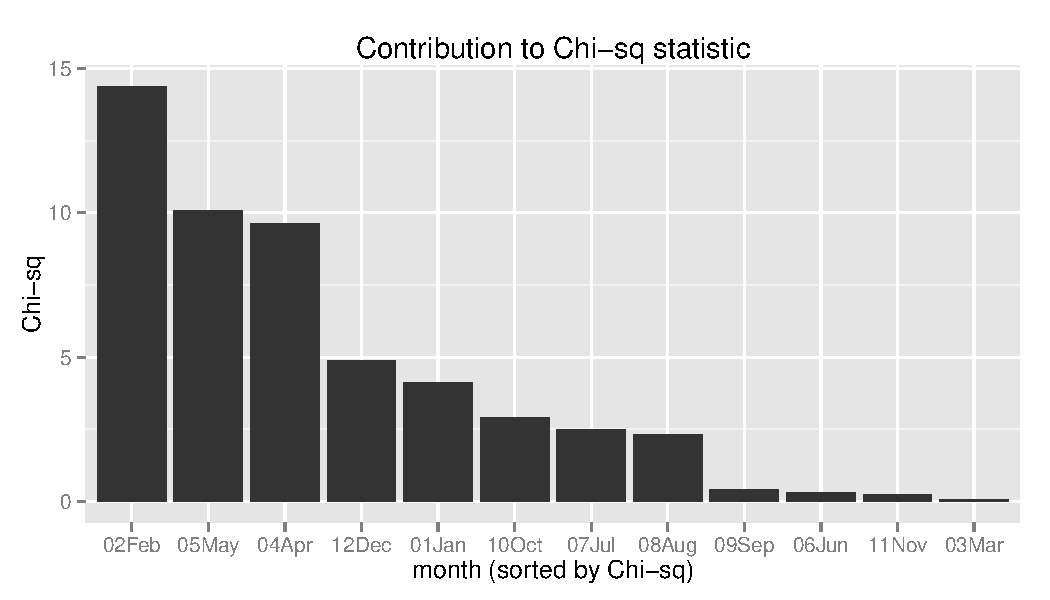
\includegraphics[width=\maxwidth]{figure/3_plot-2} 

}



\end{knitrout}

\begin{knitrout}
\definecolor{shadecolor}{rgb}{0.969, 0.969, 0.969}\color{fgcolor}\begin{kframe}
\begin{alltt}
\hlstd{b.sum1} \hlkwb{<-} \hlkwd{binom.test}\hlstd{(suicide}\hlopt{$}\hlstd{Suicides[}\hlnum{1}\hlstd{],} \hlkwd{sum}\hlstd{(suicide}\hlopt{$}\hlstd{Suicides),} \hlkwc{p} \hlstd{= suicide}\hlopt{$}\hlstd{prop.eq[}\hlnum{1}\hlstd{],} \hlkwc{alternative} \hlstd{=} \hlstr{"two.sided"}\hlstd{,} \hlkwc{conf.level} \hlstd{=} \hlnum{1}\hlopt{-}\hlnum{0.5}\hlopt{/}\hlnum{12}\hlstd{)}
\hlstd{b.sum2} \hlkwb{<-} \hlkwd{binom.test}\hlstd{(suicide}\hlopt{$}\hlstd{Suicides[}\hlnum{2}\hlstd{],} \hlkwd{sum}\hlstd{(suicide}\hlopt{$}\hlstd{Suicides),} \hlkwc{p} \hlstd{= suicide}\hlopt{$}\hlstd{prop.eq[}\hlnum{2}\hlstd{],} \hlkwc{alternative} \hlstd{=} \hlstr{"two.sided"}\hlstd{,} \hlkwc{conf.level} \hlstd{=} \hlnum{1}\hlopt{-}\hlnum{0.5}\hlopt{/}\hlnum{12}\hlstd{)}
\hlstd{b.sum3} \hlkwb{<-} \hlkwd{binom.test}\hlstd{(suicide}\hlopt{$}\hlstd{Suicides[}\hlnum{3}\hlstd{],} \hlkwd{sum}\hlstd{(suicide}\hlopt{$}\hlstd{Suicides),} \hlkwc{p} \hlstd{= suicide}\hlopt{$}\hlstd{prop.eq[}\hlnum{3}\hlstd{],} \hlkwc{alternative} \hlstd{=} \hlstr{"two.sided"}\hlstd{,} \hlkwc{conf.level} \hlstd{=} \hlnum{1}\hlopt{-}\hlnum{0.5}\hlopt{/}\hlnum{12}\hlstd{)}
\hlstd{b.sum4} \hlkwb{<-} \hlkwd{binom.test}\hlstd{(suicide}\hlopt{$}\hlstd{Suicides[}\hlnum{4}\hlstd{],} \hlkwd{sum}\hlstd{(suicide}\hlopt{$}\hlstd{Suicides),} \hlkwc{p} \hlstd{= suicide}\hlopt{$}\hlstd{prop.eq[}\hlnum{4}\hlstd{],} \hlkwc{alternative} \hlstd{=} \hlstr{"two.sided"}\hlstd{,} \hlkwc{conf.level} \hlstd{=} \hlnum{1}\hlopt{-}\hlnum{0.5}\hlopt{/}\hlnum{12}\hlstd{)}
\hlstd{b.sum5} \hlkwb{<-} \hlkwd{binom.test}\hlstd{(suicide}\hlopt{$}\hlstd{Suicides[}\hlnum{5}\hlstd{],} \hlkwd{sum}\hlstd{(suicide}\hlopt{$}\hlstd{Suicides),} \hlkwc{p} \hlstd{= suicide}\hlopt{$}\hlstd{prop.eq[}\hlnum{5}\hlstd{],} \hlkwc{alternative} \hlstd{=} \hlstr{"two.sided"}\hlstd{,} \hlkwc{conf.level} \hlstd{=} \hlnum{1}\hlopt{-}\hlnum{0.5}\hlopt{/}\hlnum{12}\hlstd{)}
\hlstd{b.sum6} \hlkwb{<-} \hlkwd{binom.test}\hlstd{(suicide}\hlopt{$}\hlstd{Suicides[}\hlnum{6}\hlstd{],} \hlkwd{sum}\hlstd{(suicide}\hlopt{$}\hlstd{Suicides),} \hlkwc{p} \hlstd{= suicide}\hlopt{$}\hlstd{prop.eq[}\hlnum{6}\hlstd{],} \hlkwc{alternative} \hlstd{=} \hlstr{"two.sided"}\hlstd{,} \hlkwc{conf.level} \hlstd{=} \hlnum{1}\hlopt{-}\hlnum{0.5}\hlopt{/}\hlnum{12}\hlstd{)}
\hlstd{b.sum7} \hlkwb{<-} \hlkwd{binom.test}\hlstd{(suicide}\hlopt{$}\hlstd{Suicides[}\hlnum{7}\hlstd{],} \hlkwd{sum}\hlstd{(suicide}\hlopt{$}\hlstd{Suicides),} \hlkwc{p} \hlstd{= suicide}\hlopt{$}\hlstd{prop.eq[}\hlnum{7}\hlstd{],} \hlkwc{alternative} \hlstd{=} \hlstr{"two.sided"}\hlstd{,} \hlkwc{conf.level} \hlstd{=} \hlnum{1}\hlopt{-}\hlnum{0.5}\hlopt{/}\hlnum{12}\hlstd{)}
\hlstd{b.sum8} \hlkwb{<-} \hlkwd{binom.test}\hlstd{(suicide}\hlopt{$}\hlstd{Suicides[}\hlnum{8}\hlstd{],} \hlkwd{sum}\hlstd{(suicide}\hlopt{$}\hlstd{Suicides),} \hlkwc{p} \hlstd{= suicide}\hlopt{$}\hlstd{prop.eq[}\hlnum{8}\hlstd{],} \hlkwc{alternative} \hlstd{=} \hlstr{"two.sided"}\hlstd{,} \hlkwc{conf.level} \hlstd{=} \hlnum{1}\hlopt{-}\hlnum{0.5}\hlopt{/}\hlnum{12}\hlstd{)}
\hlstd{b.sum9} \hlkwb{<-} \hlkwd{binom.test}\hlstd{(suicide}\hlopt{$}\hlstd{Suicides[}\hlnum{9}\hlstd{],} \hlkwd{sum}\hlstd{(suicide}\hlopt{$}\hlstd{Suicides),} \hlkwc{p} \hlstd{= suicide}\hlopt{$}\hlstd{prop.eq[}\hlnum{9}\hlstd{],} \hlkwc{alternative} \hlstd{=} \hlstr{"two.sided"}\hlstd{,} \hlkwc{conf.level} \hlstd{=} \hlnum{1}\hlopt{-}\hlnum{0.5}\hlopt{/}\hlnum{12}\hlstd{)}
\hlstd{b.sum10} \hlkwb{<-} \hlkwd{binom.test}\hlstd{(suicide}\hlopt{$}\hlstd{Suicides[}\hlnum{10}\hlstd{],} \hlkwd{sum}\hlstd{(suicide}\hlopt{$}\hlstd{Suicides),} \hlkwc{p} \hlstd{= suicide}\hlopt{$}\hlstd{prop.eq[}\hlnum{10}\hlstd{],} \hlkwc{alternative} \hlstd{=} \hlstr{"two.sided"}\hlstd{,} \hlkwc{conf.level} \hlstd{=} \hlnum{1}\hlopt{-}\hlnum{0.5}\hlopt{/}\hlnum{12}\hlstd{)}
\hlstd{b.sum11} \hlkwb{<-} \hlkwd{binom.test}\hlstd{(suicide}\hlopt{$}\hlstd{Suicides[}\hlnum{11}\hlstd{],} \hlkwd{sum}\hlstd{(suicide}\hlopt{$}\hlstd{Suicides),} \hlkwc{p} \hlstd{= suicide}\hlopt{$}\hlstd{prop.eq[}\hlnum{11}\hlstd{],} \hlkwc{alternative} \hlstd{=} \hlstr{"two.sided"}\hlstd{,} \hlkwc{conf.level} \hlstd{=} \hlnum{1}\hlopt{-}\hlnum{0.5}\hlopt{/}\hlnum{12}\hlstd{)}
\hlstd{b.sum12} \hlkwb{<-} \hlkwd{binom.test}\hlstd{(suicide}\hlopt{$}\hlstd{Suicides[}\hlnum{12}\hlstd{],} \hlkwd{sum}\hlstd{(suicide}\hlopt{$}\hlstd{Suicides),} \hlkwc{p} \hlstd{= suicide}\hlopt{$}\hlstd{prop.eq[}\hlnum{12}\hlstd{],} \hlkwc{alternative} \hlstd{=} \hlstr{"two.sided"}\hlstd{,} \hlkwc{conf.level} \hlstd{=} \hlnum{1}\hlopt{-}\hlnum{0.5}\hlopt{/}\hlnum{12}\hlstd{)}

\hlstd{b.sum}  \hlkwb{<-} \hlkwd{data.frame}\hlstd{(}
            \hlkwd{rbind}\hlstd{(} \hlkwd{c}\hlstd{(b.sum1}\hlopt{$}\hlstd{p.value, b.sum1}\hlopt{$}\hlstd{conf.int)}
                 \hlstd{,} \hlkwd{c}\hlstd{(b.sum2}\hlopt{$}\hlstd{p.value, b.sum2}\hlopt{$}\hlstd{conf.int)}
                 \hlstd{,} \hlkwd{c}\hlstd{(b.sum3}\hlopt{$}\hlstd{p.value, b.sum3}\hlopt{$}\hlstd{conf.int)}
                 \hlstd{,} \hlkwd{c}\hlstd{(b.sum4}\hlopt{$}\hlstd{p.value, b.sum4}\hlopt{$}\hlstd{conf.int)}
                 \hlstd{,} \hlkwd{c}\hlstd{(b.sum5}\hlopt{$}\hlstd{p.value, b.sum5}\hlopt{$}\hlstd{conf.int)}
                 \hlstd{,} \hlkwd{c}\hlstd{(b.sum6}\hlopt{$}\hlstd{p.value, b.sum6}\hlopt{$}\hlstd{conf.int)}
                 \hlstd{,} \hlkwd{c}\hlstd{(b.sum7}\hlopt{$}\hlstd{p.value, b.sum7}\hlopt{$}\hlstd{conf.int)}
                 \hlstd{,} \hlkwd{c}\hlstd{(b.sum8}\hlopt{$}\hlstd{p.value, b.sum8}\hlopt{$}\hlstd{conf.int)}
                 \hlstd{,} \hlkwd{c}\hlstd{(b.sum9}\hlopt{$}\hlstd{p.value, b.sum9}\hlopt{$}\hlstd{conf.int)}
                 \hlstd{,} \hlkwd{c}\hlstd{(b.sum10}\hlopt{$}\hlstd{p.value, b.sum10}\hlopt{$}\hlstd{conf.int)}
                 \hlstd{,} \hlkwd{c}\hlstd{(b.sum11}\hlopt{$}\hlstd{p.value, b.sum11}\hlopt{$}\hlstd{conf.int)}
                 \hlstd{,} \hlkwd{c}\hlstd{(b.sum12}\hlopt{$}\hlstd{p.value, b.sum12}\hlopt{$}\hlstd{conf.int)}
\hlstd{) )}

\hlkwd{names}\hlstd{(b.sum)} \hlkwb{<-} \hlkwd{c}\hlstd{(}\hlstr{"p.value"}\hlstd{,} \hlstr{"CI.lower"}\hlstd{,} \hlstr{"CI.upper"}\hlstd{)}
\hlstd{b.sum}\hlopt{$}\hlstd{Month} \hlkwb{<-} \hlstd{suicide}\hlopt{$}\hlstd{Month}
\hlstd{b.sum}\hlopt{$}\hlstd{Observed} \hlkwb{<-} \hlstd{x.table}\hlopt{$}\hlstd{obs}\hlopt{/}\hlkwd{sum}\hlstd{(x.table}\hlopt{$}\hlstd{obs)}
\hlstd{b.sum}\hlopt{$}\hlstd{EqualProp} \hlkwb{<-} \hlstd{suicide}\hlopt{$}\hlstd{prop.eq}
\hlstd{b.sum} \hlkwb{<-} \hlstd{b.sum[,}\hlkwd{c}\hlstd{(}\hlnum{4}\hlstd{,}\hlnum{1}\hlopt{:}\hlnum{3}\hlstd{,}\hlnum{5}\hlstd{,}\hlnum{6}\hlstd{)]}
\end{alltt}
\end{kframe}
\end{knitrout}

% latex table generated in R 3.1.0 by xtable 1.7-4 package
% Wed Nov 19 00:30:25 2014
\begin{table}[ht]
\centering
\begin{tabular}{rlrrrrr}
  \hline
 & Month & p.value & CI.lower & CI.upper & Observed & EqualProp \\ 
  \hline
1 & 01Jan & 0.035 & 0.076 & 0.083 & 0.080 & 0.083 \\ 
  2 & 02Feb & 0.000 & 0.073 & 0.080 & 0.076 & 0.083 \\ 
  3 & 03Mar & 0.777 & 0.079 & 0.087 & 0.083 & 0.083 \\ 
  4 & 04Apr & 0.001 & 0.085 & 0.093 & 0.089 & 0.083 \\ 
  5 & 05May & 0.001 & 0.086 & 0.093 & 0.089 & 0.083 \\ 
  6 & 06Jun & 0.563 & 0.081 & 0.088 & 0.084 & 0.083 \\ 
  7 & 07Jul & 0.101 & 0.077 & 0.084 & 0.080 & 0.083 \\ 
  8 & 08Aug & 0.114 & 0.083 & 0.090 & 0.086 & 0.083 \\ 
  9 & 09Sep & 0.509 & 0.078 & 0.086 & 0.082 & 0.083 \\ 
  10 & 10Oct & 0.077 & 0.083 & 0.090 & 0.087 & 0.083 \\ 
  11 & 11Nov & 0.612 & 0.081 & 0.088 & 0.084 & 0.083 \\ 
  12 & 12Dec & 0.021 & 0.076 & 0.083 & 0.079 & 0.083 \\ 
   \hline
\end{tabular}
\end{table}


Results from the exact binomial tests show that months Feb., May, Apr., Dec, and Jan. all have p-values less than 0.05.  Again, bases an these analysis I reject the null hypothesis in favor of the alternative; that is the suicide rate is not constant.

\section{Welsh and Breton}

\begin{knitrout}
\definecolor{shadecolor}{rgb}{0.969, 0.969, 0.969}\color{fgcolor}\begin{kframe}
\begin{alltt}
\hlkwd{prop.test}\hlstd{(}\hlkwd{c}\hlstd{(}\hlnum{76}\hlstd{,} \hlnum{57}\hlstd{),} \hlkwd{c}\hlstd{(}\hlnum{86}\hlstd{,} \hlnum{77}\hlstd{),} \hlkwc{correct} \hlstd{=} \hlnum{FALSE}\hlstd{)}
\end{alltt}
\begin{verbatim}
## 
## 	2-sample test for equality of proportions without continuity
## 	correction
## 
## data:  c(76, 57) out of c(86, 77)
## X-squared = 5.5677, df = 1, p-value = 0.0183
## alternative hypothesis: two.sided
## 95 percent confidence interval:
##  0.02437108 0.26255130
## sample estimates:
##    prop 1    prop 2 
## 0.8837209 0.7402597
\end{verbatim}
\end{kframe}
\end{knitrout}

Let $p_1$ and $p_2$ be the proportion of bilingual adults in Welsh who speak Welsh fluently and the proportion of bilingual adults in Brittany who speak Brenton fluently, respectively.  Then the null hypothesis is that both population proportions are equal, $H_0: p_1 = p_2$, agains the alternative $H_A: p_1 \ne p_2$.

The p-value for the test of equal proportions was 0.018; therefore, at the 5\% level I reject the null hypothesis in favor of the alternative.  That is the proportion of Welsh bilingual adults who speak Welsh fluently is not equal to the proportion of Brittany bilingual adults who speak Brenton fluiently.  With 95\% confidence, the proportion of Welsh bilingual adults who speak Welsh fluetnly is greater than the proportion of Brittany bilingual adults who speak Breton fluently by at least 0.024 but less than 0.263.

\section{Hawaiian blood}
\begin{knitrout}
\definecolor{shadecolor}{rgb}{0.969, 0.969, 0.969}\color{fgcolor}\begin{kframe}
\begin{alltt}
\hlstd{blood} \hlkwb{<-} \hlkwd{read.table}\hlstd{(}\hlkwc{text}\hlstd{=}\hlstr{"
Blood_Type Hawaiian   Hawaiian_White   Hawaiian_Chinese White
O 1903          4469             2206 53759
A 2490          4671             2368 50008
B 178           606              568 16252
AB 99           236              243 5001
"}\hlstd{,} \hlkwc{header}\hlstd{=}\hlnum{TRUE}\hlstd{,} \hlkwc{skip}\hlstd{=}\hlnum{1}\hlstd{)}

\hlcom{# reshape into matrix for chisq.test()}
\hlstd{blood.matrix} \hlkwb{<-} \hlkwd{matrix}\hlstd{(}\hlkwd{c}\hlstd{(blood[,}\hlnum{2}\hlstd{], blood[,}\hlnum{3}\hlstd{], blood[,}\hlnum{4}\hlstd{], blood[,}\hlnum{5}\hlstd{]),}
                  \hlkwc{ncol} \hlstd{=} \hlnum{4}\hlstd{,} \hlkwc{byrow} \hlstd{=} \hlnum{FALSE}\hlstd{,}
                  \hlkwc{dimnames} \hlstd{=} \hlkwd{list}\hlstd{(}\hlstr{"Blood_type"} \hlstd{=} \hlkwd{c}\hlstd{(}\hlstr{"O"}\hlstd{,} \hlstr{"A"}\hlstd{,} \hlstr{"B"}\hlstd{,} \hlstr{"AB"}\hlstd{),}
   \hlstr{"Ethnicity"} \hlstd{=} \hlkwd{c}\hlstd{(}\hlstr{"Hawaiian"}\hlstd{,} \hlstr{"Hawaiian_White"}\hlstd{,} \hlstr{"Hawaiian_Chinese"}\hlstd{,} \hlstr{"White"}\hlstd{)))}

\hlstd{eth.sum} \hlkwb{<-} \hlkwd{colSums}\hlstd{(blood.matrix)}
\hlstd{blood.matrix.sum} \hlkwb{<-} \hlkwd{rbind}\hlstd{(blood.matrix, eth.sum)}
\hlkwd{rownames}\hlstd{(blood.matrix.sum)} \hlkwb{<-} \hlkwd{c}\hlstd{(}\hlkwd{rownames}\hlstd{(blood.matrix),}\hlstr{"Total"}\hlstd{)}
\hlstd{blood.table} \hlkwb{<-} \hlkwd{t}\hlstd{(}\hlkwd{apply}\hlstd{(blood.matrix.sum,} \hlnum{1}\hlstd{,} \hlkwa{function}\hlstd{(}\hlkwc{x}\hlstd{) x}\hlopt{/}\hlstd{eth.sum))}
\end{alltt}
\end{kframe}
\end{knitrout}

\subsection{(15 pts) Summarize these data, focusing on comparing the proportions or percents in the 4 blood categories across the 4 ethnic groups.}

% latex table generated in R 3.1.0 by xtable 1.7-4 package
% Wed Nov 19 00:30:25 2014
\begin{table}[ht]
\centering
\begin{tabular}{r|cccc}
  \hline
 & Hawaiian & Hawaiian\_White & Hawaiian\_Chinese & White \\ 
  \hline
O & 0.407 & 0.448 & 0.410 & 0.430 \\ 
  A & 0.533 & 0.468 & 0.440 & 0.400 \\ 
  B & 0.038 & 0.061 & 0.105 & 0.130 \\ 
  AB & 0.021 & 0.024 & 0.045 & 0.040 \\ 
   \hline
Total & 1.000 & 1.000 & 1.000 & 1.000 \\ 
   \hline
\end{tabular}
\end{table}


\begin{knitrout}
\definecolor{shadecolor}{rgb}{0.969, 0.969, 0.969}\color{fgcolor}\begin{kframe}
\begin{alltt}
\hlstd{blood.stat} \hlkwb{<-} \hlstd{blood.table[}\hlnum{1}\hlopt{:}\hlnum{4}\hlstd{,]}
\hlstd{blood.stat.long} \hlkwb{<-} \hlkwd{melt}\hlstd{(blood.stat,}
                        \hlkwc{id.vars} \hlstd{=} \hlkwd{colnames}\hlstd{(blood.stat),}
                        \hlkwc{measure.vars} \hlstd{=} \hlkwd{rownames}\hlstd{(blood.stat),}
                        \hlkwc{variable.name} \hlstd{=} \hlstr{"Prop"}\hlstd{,}
                        \hlkwc{value.name} \hlstd{=} \hlstr{"Proportion"}\hlstd{)}
\hlkwd{colnames}\hlstd{(blood.stat.long)[}\hlnum{1}\hlopt{:}\hlnum{2}\hlstd{]} \hlkwb{<-} \hlkwd{c}\hlstd{(}\hlstr{"Type"}\hlstd{,} \hlstr{"Ethnicity"}\hlstd{)}

\hlkwd{library}\hlstd{(ggplot2)}
\hlstd{p.b} \hlkwb{<-} \hlkwd{ggplot}\hlstd{(blood.stat.long,} \hlkwd{aes}\hlstd{(}\hlkwc{x} \hlstd{= Ethnicity,} \hlkwc{weight} \hlstd{= Proportion))}
\hlstd{p.b} \hlkwb{<-} \hlstd{p.b} \hlopt{+} \hlkwd{geom_bar}\hlstd{()}
\hlstd{p.b} \hlkwb{<-} \hlstd{p.b} \hlopt{+} \hlkwd{facet_wrap}\hlstd{(}\hlopt{~}\hlstd{Type)}
\hlstd{p.b} \hlkwb{<-} \hlstd{p.b} \hlopt{+} \hlkwd{labs}\hlstd{(}\hlkwc{y} \hlstd{=} \hlstr{"Proportion of Blood Type"}\hlstd{)}
\hlstd{p.b} \hlkwb{<-} \hlstd{p.b} \hlopt{+} \hlkwd{theme}\hlstd{(}\hlkwc{axis.text.x} \hlstd{=} \hlkwd{element_text}\hlstd{(}\hlkwc{angle} \hlstd{=} \hlnum{15}\hlstd{))}
\hlstd{p.b}
\end{alltt}
\end{kframe}

{\centering 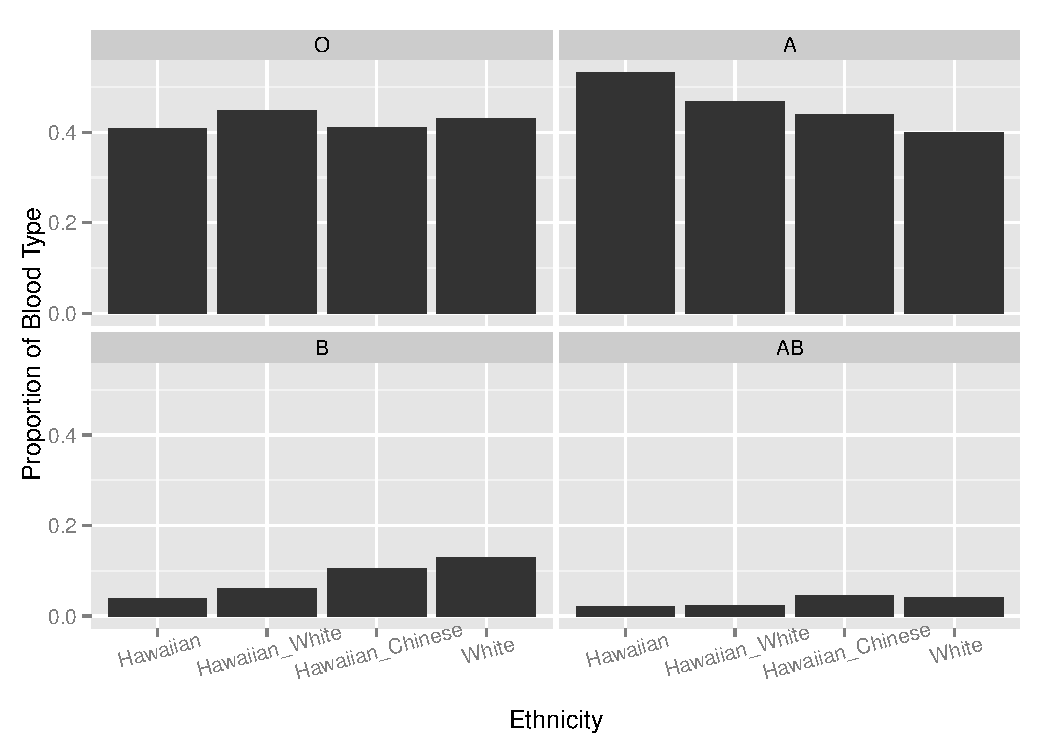
\includegraphics[width=\maxwidth]{figure/5_plot-1} 

}


\begin{kframe}\begin{alltt}
\hlstd{p.5} \hlkwb{<-} \hlkwd{ggplot}\hlstd{(blood.stat.long,} \hlkwd{aes}\hlstd{(}\hlkwc{x} \hlstd{= Type,} \hlkwc{y} \hlstd{= Proportion))}
\hlstd{p.5} \hlkwb{<-} \hlstd{p.5} \hlopt{+} \hlkwd{geom_boxplot}\hlstd{(}\hlkwc{size} \hlstd{=} \hlnum{0.75}\hlstd{,} \hlkwc{alpha} \hlstd{=} \hlnum{0.5}\hlstd{)}
\hlstd{p.5} \hlkwb{<-} \hlstd{p.5} \hlopt{+} \hlkwd{stat_summary}\hlstd{(}\hlkwc{fun.y} \hlstd{= mean,} \hlkwc{geom} \hlstd{=} \hlstr{"point"}\hlstd{,} \hlkwc{shape} \hlstd{=} \hlnum{18}\hlstd{,} \hlkwc{size} \hlstd{=} \hlnum{4}\hlstd{,}
                               \hlkwd{aes}\hlstd{(}\hlkwc{color} \hlstd{= Ethnicity),} \hlkwc{alpha} \hlstd{=} \hlnum{0.8}\hlstd{,}
                          \hlkwc{position} \hlstd{=} \hlkwd{position_jitter}\hlstd{(}\hlkwc{w} \hlstd{=} \hlnum{0.05}\hlstd{,} \hlkwc{h} \hlstd{=} \hlnum{0}\hlstd{))}
\hlstd{p.5} \hlkwb{<-} \hlstd{p.5} \hlopt{+} \hlkwd{labs}\hlstd{(}\hlkwc{y} \hlstd{=} \hlstr{"Proportion of Blood Type"}\hlstd{)}
\hlstd{p.5}
\end{alltt}
\end{kframe}

{\centering 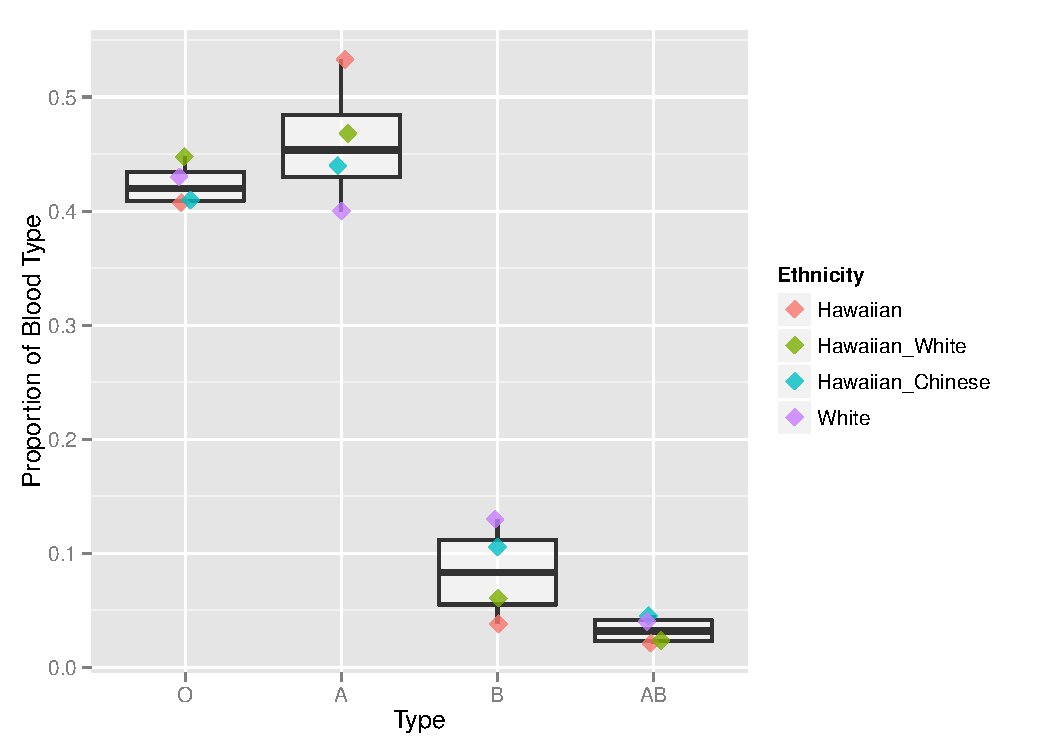
\includegraphics[width=\maxwidth]{figure/5_plot-2} 

}



\end{knitrout}

The proportions of type O and AB blood have little varation across all ethnicities and have proportions ranging from 0.407 to 0.448 and 0.021 to 0.045, respectively.  Proportions of Type A and B blood have much larger of variation across all ethnicities, with ranges from 0.400 to 0.533 and 0.038 to 0.130, respectively.  The two most common blood types for all four ethnicities were Type O and A, while types B and AB were significantly less prevalent in all ethnicities.  Hawaiians appear to have disproportionally high Type A blood while Whites appear to be disproportionally low.  Conversely, Whites appear to have a disproportionally high rate of Type B blood while Hawaiians are disproportionally low in this blood type.

\subsection{(15 pts) Is there evidence that blood type and ethnicity are associated in Hawaii? Explain.}
A test for independence of blood type and ethnicity will be implemented using the chi-squared test. The null hypothesis is that the proportion of  each blood type is consistent across ethnic groups in Hawaii $H_A: p_H = p_{HW} = p_{HC} = p_W$ against the alternative $H_A \ne H_0$ for blood types O, A, B, and AB.  The subscripts H, HW, HC, and W represent Hawaiian, Hawaiian-White, Hawaiian-Chinese, and White, respectively.

\begin{knitrout}
\definecolor{shadecolor}{rgb}{0.969, 0.969, 0.969}\color{fgcolor}\begin{kframe}
\begin{alltt}
\hlstd{chisq.5b} \hlkwb{<-} \hlkwd{chisq.test}\hlstd{(blood.matrix,} \hlkwc{correct} \hlstd{=} \hlnum{FALSE}\hlstd{)}
\hlstd{chisq.5b}
\end{alltt}
\begin{verbatim}
## 
## 	Pearson's Chi-squared test
## 
## data:  blood.matrix
## X-squared = 1078.604, df = 9, p-value < 2.2e-16
\end{verbatim}
\end{kframe}
\end{knitrout}

The Pearson chi-squared test of independence resulted in a p-value of 2.2e-16, which is much less that 0.05.  This result indicates an association between blood type and ethincity exists at the 5\% level.  The figure belows shows the observed versus expected values for each ethnicity and blood type.
\subsection{(10pts) Carry out any additional analyses that you deem relevant, and summarize your findings.
For example, there are a number of possible additional analyses that could be done here.
}
\begin{knitrout}
\definecolor{shadecolor}{rgb}{0.969, 0.969, 0.969}\color{fgcolor}

{\centering 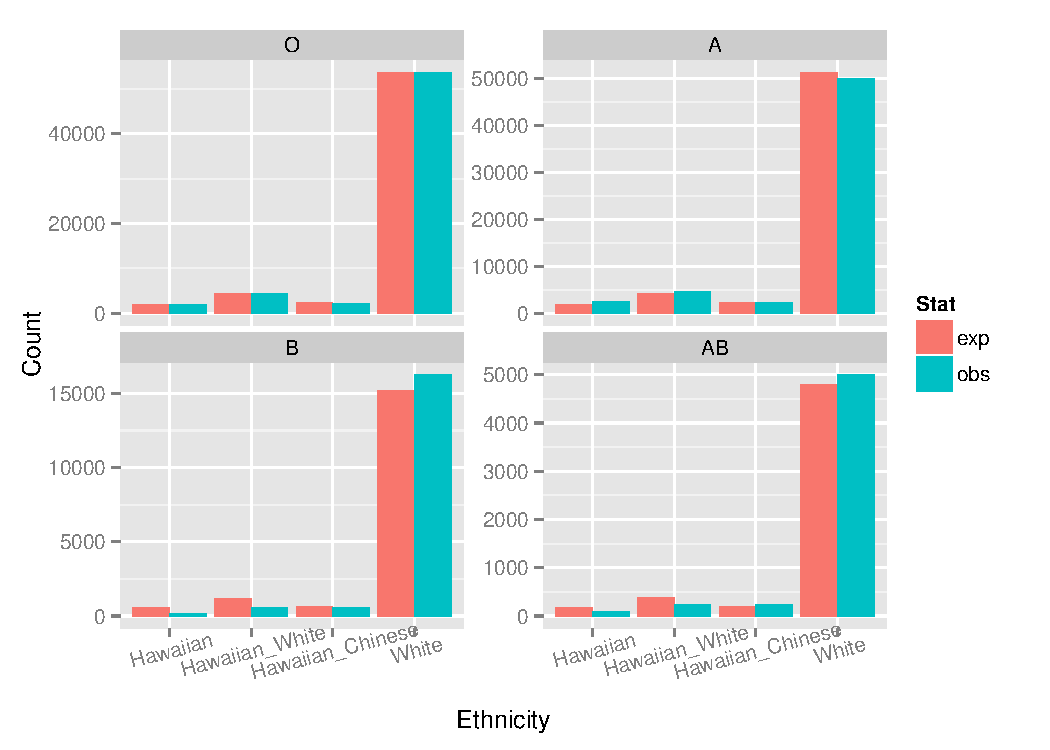
\includegraphics[width=\maxwidth]{figure/5b_table-1} 

}



\end{knitrout}

\begin{knitrout}
\definecolor{shadecolor}{rgb}{0.969, 0.969, 0.969}\color{fgcolor}\begin{kframe}
\begin{alltt}
\hlstd{blood.table.pair} \hlkwb{<-} \hlkwd{data.frame}\hlstd{(}\hlkwc{Interval} \hlstd{=} \hlkwd{rep}\hlstd{(}\hlnum{NA}\hlstd{,}\hlnum{24}\hlstd{) ,}
                          \hlkwc{CI.lower} \hlstd{=} \hlkwd{rep}\hlstd{(}\hlnum{NA}\hlstd{,}\hlnum{24}\hlstd{) ,}
                          \hlkwc{CI.upper} \hlstd{=} \hlkwd{rep}\hlstd{(}\hlnum{NA}\hlstd{,}\hlnum{24}\hlstd{) ,}
                          \hlkwc{Z} \hlstd{=} \hlkwd{rep}\hlstd{(}\hlnum{NA}\hlstd{,}\hlnum{24}\hlstd{) ,}
                          \hlkwc{p.value} \hlstd{=} \hlkwd{rep}\hlstd{(}\hlnum{NA}\hlstd{,}\hlnum{24}\hlstd{))}

\hlstd{blood.table.pair[,}\hlnum{1}\hlstd{]} \hlkwb{<-} \hlkwd{c}\hlstd{(}\hlstr{"O:p_H - p_HW"}\hlstd{,}
                     \hlstr{"O:p_H - p_HC"}\hlstd{,}
                     \hlstr{"O:p_H - p_W"}\hlstd{,}
                     \hlstr{"O:p_HW - p_HC"}\hlstd{,}
                     \hlstr{"O:p_HW - p_W"}\hlstd{,}
                     \hlstr{"O:p_HC - p_W"}\hlstd{,}

                     \hlstr{"A:p_H - p_HW"}\hlstd{,}
                     \hlstr{"A:p_H - p_HC"}\hlstd{,}
                     \hlstr{"A:p_H - p_W"}\hlstd{,}
                     \hlstr{"A:p_HW - p_HC"}\hlstd{,}
                     \hlstr{"A:p_HW - p_W"}\hlstd{,}
                     \hlstr{"A:p_HC - p_W"}\hlstd{,}

                     \hlstr{"B:p_H - p_HW"}\hlstd{,}
                     \hlstr{"B:p_H - p_HC"}\hlstd{,}
                     \hlstr{"B:p_H - p_W"}\hlstd{,}
                     \hlstr{"B:p_HW - p_HC"}\hlstd{,}
                     \hlstr{"B:p_HW - p_W"}\hlstd{,}
                     \hlstr{"B:p_HC - p_W"}\hlstd{,}

                     \hlstr{"AB:p_H - p_HW"}\hlstd{,}
                     \hlstr{"AB:p_H - p_HC"}\hlstd{,}
                     \hlstr{"AB:p_H - p_W"}\hlstd{,}
                     \hlstr{"AB:p_HW - p_HC"}\hlstd{,}
                     \hlstr{"AB:p_HW - p_W"}\hlstd{,}
                     \hlstr{"AB:p_HC - p_W"}\hlstd{)}

\hlstd{i.tab} \hlkwb{<-} \hlnum{0}
\hlkwa{for}\hlstd{(i} \hlkwa{in} \hlnum{1}\hlopt{:}\hlnum{4}\hlstd{)\{} \hlcom{#loops over blood type}
  \hlkwa{for} \hlstd{(j} \hlkwa{in} \hlnum{1}\hlopt{:}\hlnum{3}\hlstd{)\{} \hlcom{#moves first test stats}
    \hlkwa{for}\hlstd{(k} \hlkwa{in} \hlstd{(j} \hlopt{+} \hlnum{1}\hlstd{)}\hlopt{:}\hlnum{4}\hlstd{) \{} \hlcom{#moves second test stat}
      \hlstd{i.tab} \hlkwb{<-} \hlstd{i.tab} \hlopt{+} \hlnum{1}
      \hlstd{blood.summary} \hlkwb{<-} \hlkwd{prop.test}\hlstd{(}\hlkwd{rbind}\hlstd{(}\hlkwd{c}\hlstd{(blood.matrix.sum[i,j], blood.matrix.sum[}\hlnum{5}\hlstd{,j]} \hlopt{-} \hlstd{blood.matrix.sum[i,j]),}
                           \hlkwd{c}\hlstd{(blood.matrix.sum[i,k], blood.matrix.sum[}\hlnum{5}\hlstd{,k]} \hlopt{-} \hlstd{blood.matrix.sum[i,k])),}
                           \hlkwc{correct} \hlstd{=} \hlnum{FALSE}\hlstd{,} \hlkwc{conf.level} \hlstd{=} \hlnum{1} \hlopt{-} \hlnum{0.05}\hlopt{/}\hlnum{6}\hlstd{)}

      \hlstd{blood.table.pair[i.tab,} \hlnum{2}\hlopt{:}\hlnum{5}\hlstd{]} \hlkwb{<-} \hlkwd{c}\hlstd{(blood.summary}\hlopt{$}\hlstd{conf.int[}\hlnum{1}\hlstd{],}
                                   \hlstd{blood.summary}\hlopt{$}\hlstd{conf.int[}\hlnum{2}\hlstd{],}
                                   \hlkwd{sign}\hlstd{(}\hlopt{-}\hlkwd{diff}\hlstd{(blood.summary}\hlopt{$}\hlstd{estimate))} \hlopt{*} \hlstd{blood.summary}\hlopt{$}\hlstd{statistic}\hlopt{^}\hlnum{0.5}\hlstd{,}
                                   \hlstd{blood.summary}\hlopt{$}\hlstd{p.value)}
    \hlstd{\}}
  \hlstd{\}}
\hlstd{\}}
\end{alltt}
\end{kframe}
\end{knitrout}

% latex table generated in R 3.1.0 by xtable 1.7-4 package
% Wed Nov 19 00:30:26 2014
\begin{table}[ht]
\centering
\begin{tabular}{r|c|cccc}
  \hline
 & Interval & CI.lower & CI.upper & Z & p.value \\ 
  \hline
1 & O:p\_H - p\_HW & -0.063 & -0.017 & -4.575 & 0.000 \\ 
  2 & O:p\_H - p\_HC & -0.028 & 0.024 & -0.220 & 0.826 \\ 
  3 & O:p\_H - p\_W & -0.042 & -0.003 & -3.051 & 0.002 \\ 
  4 & O:p\_HW - p\_HC & 0.016 & 0.060 & 4.540 & 0.000 \\ 
  5 & O:p\_HW - p\_W & 0.004 & 0.031 & 3.437 & 0.001 \\ 
  6 & O:p\_HC - p\_W & -0.038 & -0.002 & -2.954 & 0.003 \\ 
  7 & A:p\_H - p\_HW & 0.042 & 0.089 & 7.363 & 0.000 \\ 
  8 & A:p\_H - p\_HC & 0.067 & 0.120 & 9.352 & 0.000 \\ 
  9 & A:p\_H - p\_W & 0.114 & 0.153 & 18.206 & 0.000 \\ 
  10 & A:p\_HW - p\_HC & 0.006 & 0.050 & 3.348 & 0.001 \\ 
  11 & A:p\_HW - p\_W & 0.054 & 0.082 & 13.307 & 0.000 \\ 
  12 & A:p\_HC - p\_W & 0.022 & 0.058 & 5.825 & 0.000 \\ 
  13 & B:p\_H - p\_HW & -0.032 & -0.013 & -5.663 & 0.000 \\ 
  14 & B:p\_H - p\_HC & -0.081 & -0.054 & -12.854 & 0.000 \\ 
  15 & B:p\_H - p\_W & -0.100 & -0.084 & -18.534 & 0.000 \\ 
  16 & B:p\_HW - p\_HC & -0.057 & -0.032 & -9.968 & 0.000 \\ 
  17 & B:p\_HW - p\_W & -0.076 & -0.062 & -20.151 & 0.000 \\ 
  18 & B:p\_HC - p\_W & -0.036 & -0.013 & -5.256 & 0.000 \\ 
  19 & AB:p\_H - p\_HW & -0.009 & 0.004 & -0.922 & 0.356 \\ 
  20 & AB:p\_H - p\_HC & -0.033 & -0.015 & -6.601 & 0.000 \\ 
  21 & AB:p\_H - p\_W & -0.025 & -0.013 & -6.491 & 0.000 \\ 
  22 & AB:p\_HW - p\_HC & -0.030 & -0.013 & -7.311 & 0.000 \\ 
  23 & AB:p\_HW - p\_W & -0.021 & -0.012 & -8.145 & 0.000 \\ 
  24 & AB:p\_HC - p\_W & -0.002 & 0.013 & 1.874 & 0.061 \\ 
   \hline
\end{tabular}
\end{table}



Comparisons for each blood type across ethnicities with the Bonferroni adjustment to account for multiple comparisons was performed.  Within each blood type there were 6 possible comparisons; therefore, with an overall Family Error Rate of 0.05, the individual hypothese tests were performed at the 0.008 level.  This analysis resulted in identifying which
pairs have significant differences and the 99.2\% confidence interval of those differences.  All pairs showed a significant difference at the 0.8\% level except for Type O:$p_H - p_{HC}$, Type AB:$p_H - p_{HW}$, and Type AB:$p_{HC} - p_W$.

Some additional analyses that could be done include an analysis of variance and pairwise analysis of blood types within an ethnicity.

\end{document}
